% COLING 2027 (via ACL Rolling Review, 2026-10-12) — first draft, 2026-10-08.
% Frame: docs/checkpoints/paper_drafts/coling_frame_proposal.md (v2, user-chosen positive opening).
% Every number in the text is read from a product under docs/analysis/ ; the source is named in a
% comment next to it. Figures: scripts/analysis/figures/coling/make_figures.py.
% ARR page limit (8 pages long paper) and COLING-specific CFP details: NOT YET VERIFIED.
\documentclass[11pt]{article}
\usepackage[review]{acl}   % [review] anonymises and adds line numbers; [final] is the default

\usepackage{times}
\usepackage{latexsym}
\usepackage[T1]{fontenc}
\usepackage[utf8]{inputenc}
\usepackage{microtype}
\usepackage{inconsolata}
\usepackage{graphicx}
\usepackage{booktabs}
\usepackage{array}
\usepackage{amsmath,amssymb}
\usepackage{xcolor}

\graphicspath{{figures/}}
\setcounter{topnumber}{3}
\setcounter{bottomnumber}{2}
\setcounter{totalnumber}{4}
\renewcommand{\topfraction}{0.9}
\renewcommand{\bottomfraction}{0.5}
\renewcommand{\textfraction}{0.07}
\renewcommand{\floatpagefraction}{0.75}

\newcommand{\todo}[1]{{\color{red!75!black}\bfseries[TODO: #1]}}
\newcommand{\pp}{\,pp}
\newcommand{\SoM}{SoM}
\newcommand{\PSoM}{P-SoM}

\title{Text, Screenshots, or Both?\\Representation Value and Task Routing in Web Agents}

\begin{document}
\maketitle

\begin{abstract}
A web agent can read a page as text, look at a screenshot, or do both, and deployments usually fix one choice for every task. We measure that choice across three sites of VisualWebArena and WebArena with four vision-language backbones, using text-only variants as controls and rerunning identical conditions to see which differences survive.
% sources: routing_three_arm, visual_intent_routing, task_mode_interaction_null, routing_gain_upper_bounds
Three findings separate questions that are usually merged. First, no observation choice is best everywhere, and the screenshot has a real, reproducible value that is predictable in advance on one site: a zero-cost rule over the task text picks out classifieds tasks on which adding the screenshot alone raises success by 25--30 points for the two strongest backbones (11 for a 4B model), and the gap reappears on a full rerun. Second, which representation suits which task is a reproducible property of the task, beyond an additive model of task difficulty, yet a single run measures it with reliability of only 0.31--0.50. Third, two lightweight routers that choose a representation per task from pre-run features, with their operating point fixed on training data, show no reliable gain over the fixed choices and their random mixtures. We describe the rerun-controlled protocol that keeps these three quantities apart.
\end{abstract}

\section{Introduction}\label{sec:intro}

An agent that operates a website has to perceive it, and the two standard ways are complementary in principle: the page's text (an accessibility tree) is precise and cheap, a screenshot shows what the text omits. A third option fuses them, overlaying numbered marks on the screenshot and listing the marked elements as text \citep{yang2023som,koh2024visualwebarena}. Practitioners typically pick one of the three for a whole deployment. The question this paper asks is the one that choice raises: \emph{is the choice worth making per task, and can it be made?}

Answering it requires keeping apart three quantities that a single leaderboard number merges:
\begin{enumerate}\setlength{\itemsep}{0pt}
  \item \textbf{Representation value}: does the screenshot change success, holding everything else fixed?
  \item \textbf{Preference reliability}: when one representation beats another on a task, is that a stable property of the task, or a property of one run?
  \item \textbf{Routing gain}: can a policy that chooses per task, using only what is known before it runs, beat the fixed choices?
\end{enumerate}
A hindsight ceiling picks, for each task, whichever representation happened to succeed. However large, it answers none of them, because it rewards run-to-run luck as much as structure. We therefore rerun identical conditions and read every comparison against what a rerun alone changes.

\paragraph{Findings.}
(i) No choice wins everywhere: the fused mode leads on classifieds, text leads on WebArena reddit, and the order reverses across backbones (\S\ref{sec:deploy}).
(ii) The screenshot has a specific value that can be isolated and predicted: with the text payload and prompt held fixed, adding the screenshot raises success on the classifieds tasks a zero-cost intent rule flags by 25--30 points for the two strongest backbones (11 for a 4B model), against 5--10 on the other tasks; the effect reproduces on a full rerun and is larger for the stronger backbones we tested. On reddit the same rule finds nothing (\S\ref{sec:screenshot}).
(iii) Per-task preferences between representations are reproducible beyond an additive difficulty model: a no-interaction null conditioned on every task's and every mode's success count is rejected in every fully rerun cell. Yet a single run measures them with reliability 0.31--0.50, and a decision study projects that labels averaged over two to three runs would pass 0.5 (\S\ref{sec:preference}).
(iv) Two lightweight routers that fix their operating point on training data show no reliable gain over the fixed representations and their random mixtures; the one hindsight opportunity that passes its null comes from a router that only decides which tasks deserve the expensive mode, holds under billed cost only, and is not captured without looking at test outcomes (\S\ref{sec:routing}).

\paragraph{Contributions.}
A rerun-controlled measurement of text, screenshot and fused observation across three sites and four backbones, with text-only ablations that isolate the screenshot; a matched estimate of the screenshot's value and an ex-ante rule that predicts it on one site; a test of whether per-task representation preferences are reproducible, with a decision study of how many runs a reliable label needs; and a deployable-policy comparison against fixed choices \emph{and their random mixtures}, which is the comparison a routing claim has to win; we take this baseline from model-routing benchmarks and apply it to observation choice (\S\ref{sec:method}).

\section{Setup}\label{sec:setup}

\paragraph{Sites and tasks.} We use three sites of VisualWebArena \citep{koh2024visualwebarena} --- classifieds (224 scored tasks), reddit (203) and shopping (432) --- and the reddit site of WebArena \citep{zhou2024webarena} (104 tasks, those all observation modes ran). VWA-reddit and WA-reddit are different task sets on the same application, so they are not two independent benchmarks. Scored sets are the collected tasks minus protocol exclusions written as rules over task configuration (Appendix~\ref{app:universe}).

\paragraph{Backbones.} B0 = Qwen3-VL-235B (API-served), B1 = Qwen3-VL-4B and B2 = Gemma-3-4B (both served locally), and B5 = GPT-5.6 (API, classifieds only). A \emph{cell} is one site $\times$ backbone pair; the eight cells with every observation mode are VWA-classifieds and VWA-reddit $\times$ \{B0, B1, B2\} and WA-reddit $\times$ \{B0, B1\}. B5-classifieds and the two shopping cells extend them (\S\ref{sec:screenshot}, \S\ref{sec:routing}) and are never pooled with the eight.

\paragraph{One plain agent.} One model call per step emits a thought, an action and its arguments; the prompt holds the instruction, the mode's system prompt, the last eight steps and the current observation. There is no planner, memory, reflection or retry policy, so a difference between conditions is a difference of observation, not of scaffold. Episodes stop at 30 steps.

\paragraph{Observation modes.} The deployment question has three answers: \textbf{DOM} (the page's accessibility tree as text), \textbf{Vision} (the raw screenshot, with an empty text payload) and \textbf{\SoM} (a set-of-marks screenshot plus the list of marked elements as text; \citealp{yang2023som}). Three further modes carry no screenshot and serve as controls; the one used throughout is \textbf{\PSoM}, which is \SoM\ with the screenshot removed --- same marks, same prompt --- so \SoM$-$\PSoM\ isolates the image (Appendix~\ref{app:modes} lists all six). ``Text'' modes withhold the \emph{page} screenshot only: a reference image that is part of the task (``find this item'') is given in every mode.

\paragraph{Reruns.} We reran identical conditions, 24 registered same-condition pairs in all; in three cells --- VWA-classifieds B0, VWA-reddit B0 and WA-reddit B1 --- every mode was run twice. A rerun uses the same tasks, code and site reset, so what it changes is what one run of the agent does not determine.

\paragraph{Scoring and cost.} The evaluators are binary. Cost is the per-episode billed cost: an API invoice for B0 and B5, a token-priced electricity estimate for B1 and B2. The two kinds are ordered within a cell, never pooled across; \S\ref{sec:routing} repeats the routing analysis under GPU-time and wall-clock cost.

\section{No observation choice is best everywhere}\label{sec:deploy}

\begin{figure}[t]
  \centering
  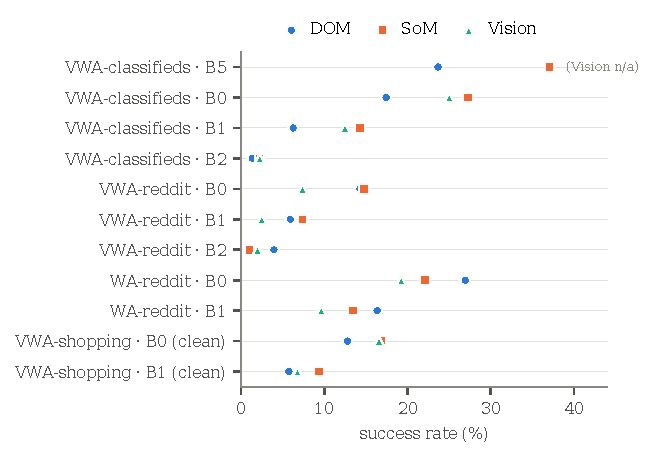
\includegraphics[width=\columnwidth]{fig_deploy}
  \caption{Success rate of the three deployment choices per cell. Shopping cells drop the tasks touched by a known harness defect in any mode (\S\ref{sec:setup}, Appendix~\ref{app:harness}); B5's Vision run is excluded for a coordinate-contract defect. Source: \texttt{routing\_three\_arm}, \texttt{routing\_extension\_cells}.}
  \label{fig:deploy}
\end{figure}

Figure~\ref{fig:deploy} shows the three deployment choices side by side. On classifieds the fused mode is the best of the three for B0, B1 and GPT-5.6 (B2 solves too few tasks to order the modes), and the margin over text is not small: \SoM$-$DOM is +9.82\pp\ [+3.57, +16.07] for B0 and +8.04\pp\ [+3.57, +12.95] for B1 (paired task bootstrap). % fusion_premium
On WebArena reddit the order flips and text leads (\SoM$-$DOM $-4.81$\pp\ for B0 and $-2.88$\pp\ for B1, both intervals crossing zero), and on VWA-reddit the weakest backbone does worse with the fused mode ($-2.96$\pp\ [$-5.91$, $-0.49$]), but three of its eight DOM successes were credited although the episode never visited the target forum, whose subscription an earlier episode had made; without them the gap is $-1.48$\pp\ [$-3.45$, $+0.49$] (Appendix~\ref{app:harness}). % fusion_premium, leakage_sensitivity
On shopping the fused mode is best or tied with Vision, on the filtered and on the full task sets (Figure~\ref{fig:deploy}, Table~\ref{tab:cells}).

Two cautions keep this descriptive. Cells on the same site share their tasks, so the eight are not eight independent replications. And the screenshot-free modes are four, not one: a maximum over four text variants against a single screenshot mode would be a selection effect, so the comparison here takes one representative per deployment class, as practitioners do.

What this section establishes is only that the choice matters and depends on the workload. Whether it can be made per task is the subject of the rest of the paper.

\section{The screenshot has a value that can be isolated and predicted}\label{sec:screenshot}

\begin{figure}[t]
  \centering
  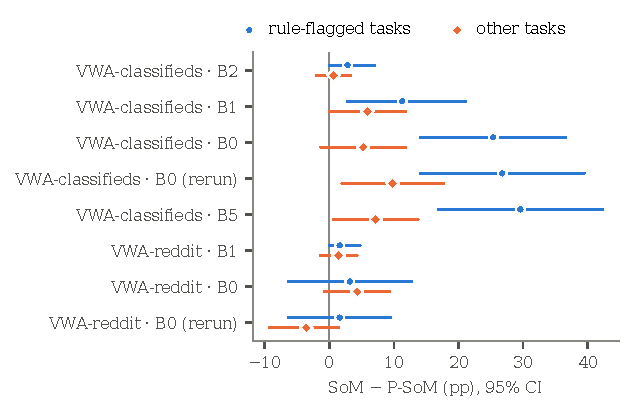
\includegraphics[width=\columnwidth]{fig_screenshot}
  \caption{Value of the screenshot alone (\SoM$-$\PSoM: same marks, same prompt) on the tasks a zero-cost intent rule flags, against the other tasks. Classifieds is out-of-sample for the rule. ``Rerun'' is a full repeat of both modes. VWA-reddit B2 is omitted: neither \SoM\ nor \PSoM\ solves a flagged task. Source: \texttt{visual\_intent\_routing}.}
  \label{fig:screenshot}
\end{figure}

\paragraph{A matched contrast.} Comparing Vision with DOM changes two things at once --- the image and the text the agent receives. \SoM\ and \PSoM\ differ only in the annotated screenshot, so their difference is the value of the image alone. \citet{chi2024elementordering} already compared screenshot-plus-text with text only on a subset of VisualWebArena tasks for one backbone (50.0\% against 46.3\%, without set-of-marks); we hold the set-of-marks text and prompt fixed, use four backbones and full task sets, rerun the contrast, and ask \emph{where} the image pays off.

\paragraph{An ex-ante rule.} A regular expression over the task intent flags tasks that ask about an image, a photo, a colour or a count of things shown, excluding tasks that already carry a reference image (Appendix~\ref{app:rule}). It reads only the task configuration: no model call and no episode. It was written as a reddit failure-diagnosis pattern a week before it was first used to partition tasks, and its classifieds hits were never inspected, so classifieds is out-of-sample for it.

\paragraph{Result.} On the 71 classifieds tasks it flags, the screenshot raises success by +25.35\pp\ [+14.08, +36.62] for B0, against +5.23\pp\ on the other 153 tasks (Figure~\ref{fig:screenshot}). % visual_intent_routing ext cls_B0
The effect reproduces on a full rerun of both modes (+26.76\pp\ [+14.08, +39.44], from 23 against 4 successes), % ext cls_B0_rerun
and it is larger for the stronger backbones we tested: +2.82\pp\ for B2, +11.27\pp\ for B1, +25.35\pp\ for B0 and +29.58\pp\ [+16.90, +42.25] for GPT-5.6 (whose parser let some actions through beyond the step budget, in both modes alike; Appendix~\ref{app:harness}). The backbones differ in more than capability, so this is an association across the four we ran, not a scaling law. % ext cls_B2/B1/B0/B5
On VWA-reddit the same rule flags 63 tasks and separates nothing: +3.17\pp\ on flagged tasks against +4.29\pp\ elsewhere for B0, +1.59\pp\ against $-3.57$\pp\ on its rerun. % ext red_B0, red_B0_rerun
On shopping the flagged tasks carry at most five successes per mode, too few to read, and on WebArena the rule flags only 5 of 104 tasks.

\paragraph{Reading.} Where the screenshot pays off on classifieds is predictable before anything runs, and it pays off more for stronger models; on reddit it is not. The screenshot's value is therefore real and partly foreseeable, but site-specific: it is a statement about a kind of task, not a general law. It is also not a router. On these tasks the fused mode already contains the screenshot, so switching between DOM and Vision by this rule cannot beat simply using \SoM; what remains open is whether \emph{individual} tasks have stable preferences beyond such task types, which is the question of \S\ref{sec:preference}.

\section{Per-task preferences are real, but one run cannot measure them}\label{sec:preference}

\S\ref{sec:screenshot} found structure at the level of task \emph{types}. Routing per task needs more: that an individual task prefers one representation over another, beyond being easy or hard, and that this preference is stable enough to learn from.

\paragraph{A null without task-by-mode structure.} In the three cells where every mode was run twice, let $Y_{imr}\in\{0,1\}$ be the outcome of task $i$ under mode $m$ in run $r$. Under
\[
  \operatorname{logit}\Pr(Y_{imr}=1) = a_i + b_{mr},
\]
every task has its own difficulty and every (mode, run) column its own easiness, but there is no persistent task-by-mode interaction. This is the Rasch structure that item-response routers use to model difficulty \citep{song2025irtrouter}; here it is the null, and the question is what lies beyond it. The row and column sums are sufficient for this model, so conditional on them every 0/1 matrix with those margins is equally likely; we approximate that conditional null by curveball Markov-chain sampling \citep{strona2014curveball}, fitting nothing. The statistic is the reproducible part of the interaction, $\hat\sigma^2_{\text{int}} = (\mathrm{MS}_{\text{int}} - \mathrm{MS}_{\text{err}})/2$ from the two-way task $\times$ mode ANOVA with two runs: the run-to-run covariance of each task's mode profile.

\paragraph{Result.} Over the three deployment modes the interaction exceeds the null in all three cells (classifieds B0 $\hat\sigma^2_{\text{int}}=0.033$ against a null 95th percentile of 0.015; reddit B0 0.018 against 0.009; WebArena-reddit B1 0.030 against 0.014; $p\le 0.002$ each, Holm across cells). % routing_three_arm null_cells
Over all six modes the same holds (Appendix~\ref{app:sixarm}). Preferences between representations are therefore a reproducible property of tasks that an additive difficulty model does not capture. The test does not say what the extra structure is: a task-specific preference and a mode whose success responds more steeply to difficulty than another's both reject this null, and only the first is a representation preference in the narrow sense.

\begin{figure}[t]
  \centering
  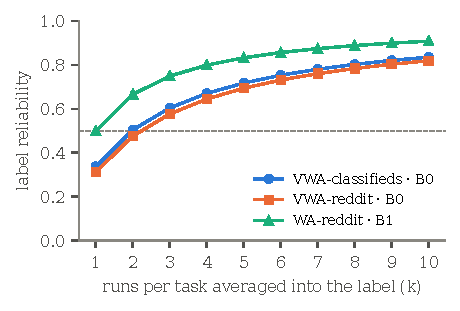
\includegraphics[width=\columnwidth]{fig_dstudy}
  \caption{Decision study for the three deployment modes: reliability of a task-by-mode label averaged over $k$ runs, $\sigma^2_{\text{int}}/(\sigma^2_{\text{int}} + \sigma^2_{\text{err}}/k)$. A single run gives 0.31--0.50. Source: \texttt{routing\_three\_arm}.}
  \label{fig:dstudy}
\end{figure}

\paragraph{But a single run measures them poorly.} The same decomposition gives, in the sense of a generalisability decision study \citep{brennan2001generalizability}, the reliability of a task's mode profile averaged over $k$ runs (Figure~\ref{fig:dstudy}). From one run it is 0.34, 0.31 and 0.50 in the three cells; the projection crosses 0.5 at two to three runs (bootstrap ranges 2--4, 2--7 and 1--3). Over six modes it is lower still, 0.14--0.46, with up to six runs projected. This is the reliability of the interaction profile, not of a router's chosen arm, so it bounds how noisy single-run training labels are rather than predicting when a router starts to win. % routing_three_arm, task_mode_interaction_null
The preferences also persist where they can be observed directly: over all six modes, taking for each task the cheapest mode that succeeded on one run and scoring that choice on the rerun beats the fixed-mode frontier by 2.4--10.5 points on reddit B0 and WebArena-reddit B1. % routing_crossrun_template_validation diagnostic
That choice uses the task's own label, which no deployment has, so it measures persistence, not an attainable policy.

The routing target thus exists, and a training set built from single runs labels it with a reliability between a third and a half.

\section{Deployable routers do not convert the signal}\label{sec:routing}

\paragraph{The comparison a router must win.} A router that sends some tasks to an expensive mode and others to a cheap one trades success for cost. Beating every fixed mode on both axes is too strict, but beating the fixed modes one at a time is too lenient: sending a random share of tasks to each of two modes is also a deployable policy. We therefore compare against the \emph{frontier of the fixed modes and all their random mixtures} --- the upper concave envelope of the fixed points in the (cost, success) plane, the non-decreasing convex hull that model-routing benchmarks use as a baseline \citep{hu2024routerbench,jitkrittum2025uniroute} --- and report how far above it a router reaches.

\paragraph{Routers.} Two constructions use 18 features available before a task runs: 14 intent-keyword indicators, the intent length, and three statistics of the first page. \emph{Per-arm heads} fit one logistic success model per mode and send a task to the cheapest mode whose predicted success clears a threshold. \emph{Triage} predicts whether any mode can solve the task, sends predicted-hopeless tasks to the cheapest mode and the rest to the best one. All predictions are out-of-fold (task-held-out five-fold).

\begin{table*}[t]
\centering\small
\setlength{\tabcolsep}{6pt}
\begin{tabular}{@{}llrr@{}}
\toprule
cells & policy & curve max (p) & deployable [5\%, 95\%] \\
\midrule
3 arms, 8 cells pooled & per-arm heads & +0.86 (0.072) & +0.23 [$-$2.20, +0.22] \\
 & triage & +1.69 (0.001) & +0.59 [$-$1.53, +1.23] \\
\addlinespace[2pt]
6 arms, 8 cells pooled & per-arm heads & +0.67 (0.252) & $-$0.38 [$-$3.20, $-$0.14] \\
 & triage & +1.24 (0.043) & $-$0.39 [$-$2.42, +0.81] \\
\addlinespace[2pt]
GPT-5.6, classifieds (5 arms) & per-arm heads & +0.45 (0.768) & $-$2.45 [$-$8.61, +4.24] \\
 & triage & +3.86 (0.127) & $-$1.63 [$-$6.70, +5.74] \\
\addlinespace[2pt]
Shopping B0, clean (3 arms) & per-arm heads & +1.14 (0.062) & $-$0.18 [$-$2.45, +2.02] \\
 & triage & +0.20 (0.496) & $-$0.87 [$-$2.63, +1.37] \\
\addlinespace[2pt]
Shopping B0, all tasks (3 arms) & per-arm heads & +1.09 (0.049) & +1.30 [$-$2.31, +1.85] \\
 & triage & +0.18 (0.541) & $-$0.05 [$-$2.14, +1.45] \\
\addlinespace[2pt]
Shopping B1, clean (6 arms) & per-arm heads & +1.11 (0.143) & +0.56 [$-$4.69, +0.88] \\
 & triage & +1.63 (0.158) & +1.19 [$-$4.10, +1.57] \\
\addlinespace[2pt]
Shopping B1, all tasks (6 arms) & per-arm heads & +0.48 (0.169) & $-$0.43 [$-$2.78, +0.73] \\
 & triage & +0.69 (0.289) & +0.40 [$-$2.02, +2.02] \\
\bottomrule
\end{tabular}
\caption{Routing gain over the fixed arms and their random mixtures, in SR points. \emph{Curve max}: the best point of an out-of-fold curve, chosen after seeing test outcomes, with its label-shuffle $p$ (pooled rows: max over a normalised budget). \emph{Deployable}: the operating point chosen on training folds only, task bootstrap. Sources: \texttt{routing\_three\_arm}, \texttt{representation\_routing\_frontier}, \texttt{routing\_gain\_upper\_bounds}, \texttt{routing\_extension\_cells}.}
\label{tab:routing}
\end{table*}


\paragraph{Room above the frontier exists, and it is difficulty.} Sweeping each router's threshold traces a curve. Over the three deployment modes, the triage curve pooled over the eight cells rises 1.69 points above the frontier at low budget, which a label-shuffle null that refits the whole curve does not produce ($p=0.001$; Table~\ref{tab:routing}). The per-arm heads reach 0.86 points ($p=0.072$). Triage does not choose a representation for a task; it decides which tasks are not worth the expensive mode. The room that exists is the difficulty lever, not representation fit.

\paragraph{A deployable router does not capture it.} A curve's best point is chosen after seeing test outcomes. When the operating point is instead chosen on training folds only, the pooled gain is +0.23 points for per-arm heads and +0.59 for triage, and neither interval excludes zero (Table~\ref{tab:routing}). Over all six modes the deployable per-arm router sits significantly \emph{below} the frontier ($-0.38$; 95\% upper bound $-0.14$). % routing_gain_upper_bounds pooled
The pattern holds for the strongest backbone: for GPT-5.6 on classifieds, where the screenshot's value was largest (\S\ref{sec:screenshot}), the deployable routers lose 1.6--2.5 points; on both shopping cells they stay within 1.2 points of the frontier.

\paragraph{Robustness.} Holding tasks of the same template out together lowers the six-mode per-arm router's mean deployable gain from $-0.38$ to $-1.60$ points, and fitting on one run and scoring on its rerun gives point estimates of both signs whose intervals all include zero (Appendix~\ref{app:robust}). % routing_crossrun_template_validation
Repricing cost as GPU time or wall-clock time leaves the frontier result unchanged, but changes \emph{which} single cell's triage curve passes a per-cell Holm correction, so no single-cell result is quoted here. % §545
One of the three-mode intervals (per-arm heads, pooled) has an upper end below its point estimate, a sign that the bootstrap of a policy with a selected threshold is biased; we read these intervals as magnitudes, not as tests.

\section{A protocol for multi-representation claims}\label{sec:method}

The three quantities of \S\ref{sec:intro} came apart because each was measured against its own control. We suggest the same four steps for any claim that choosing among several agent configurations per task would pay.

\begin{enumerate}\setlength{\itemsep}{1pt}
  \item \textbf{Report reruns per arm and per cell}, not one flip rate or one resolution threshold for a whole study: in our data a rerun changes between 0 and 14\% of outcomes depending on arm and cell (Appendix~\ref{app:sixarm}).
  \item \textbf{Isolate the component of interest with a matched ablation} (here \SoM$-$\PSoM, which removes only the screenshot) before attributing a difference to it.
  \item \textbf{Test for per-task structure against a null that conditions on difficulty}, and use a decision study to say how many runs per task make the label reliable. A single-run oracle is not a ceiling a router can reach.
  \item \textbf{Score a deployable policy, operating point chosen on training data, against the fixed arms and their random mixtures}, never only against the best single arm or a hindsight curve.
\end{enumerate}

Applied here, the protocol says the screenshot is worth paying for on a predictable class of classifieds tasks, that per-task representation preferences are reproducible but single-run labels measure them with reliability of a third to a half, and that with such labels and pre-flight features the routers we tested do not reliably beat choosing one representation, or a fixed mixture, for the whole workload.

\section{Related work}\label{sec:related}
\todo{chunk 3: only citations already in paper.bib.}

\section*{Limitations}

\paragraph{Coverage of reruns.} Only three cells have every mode run twice, two with the same backbone; the preference test and decision study (\S\ref{sec:preference}) rest on them. Five of the eleven cells have no rerun of any mode.

\paragraph{Breadth.} VWA-reddit and WA-reddit are task sets on the same application, so the study covers three applications, not four benchmarks. GPT-5.6 was run on classifieds only, and its Vision run is excluded for a coordinate-contract defect; a parser defect also let it take actions beyond the 30-step budget in every mode (Appendix~\ref{app:harness}). The ex-ante rule of \S\ref{sec:screenshot} works on classifieds only.

\paragraph{Shopping filtering.} Dropping tasks touched by the search-box defect keeps the comparison between modes clean, but the dropped tasks are mostly search tasks, so the filtered cells read a different task mix; unfiltered results are reported alongside.

\paragraph{What the routing result does not show.} The routers use 18 pre-flight features and logistic models; richer features, language-model routers or multiple runs per training task may do better. The result is that, with single-run labels and these features, the routers do not beat the fixed choices and their mixtures --- not that per-task routing is impossible. Step-level switching is out of scope.

\paragraph{Exploratory analyses.} The preference test, frontier comparisons and bounds were designed after the runs were collected. Each family states its multiplicity correction; the bootstrap intervals for policies with a selected threshold are read as magnitudes, not tests.

\paragraph{Cost.} API invoices and electricity estimates are different quantities and are never pooled; local cost depends on the pricing basis, which is why \S\ref{sec:routing} repeats the analysis under GPU time and wall-clock time.


\bibliography{paper}

\appendix
\section{Task universes and exclusions}\label{app:universe}
\todo{chunk 3}
\section{The six observation modes}\label{app:modes}
\todo{chunk 3}
\section{The intent rule}\label{app:rule}
\todo{chunk 3}
\section{Harness defects and how cells were filtered}\label{app:harness}
\todo{chunk 3}


\end{document}
